% LaTeX template for MICS papers
% To Run:  pdflatex Sample.tex

\documentclass[12pt]{article}


\setlength{\oddsidemargin}{0in}
\setlength{\evensidemargin}{0in}
\setlength{\topmargin}{0in}
\setlength{\headheight}{0in}
\setlength{\headsep}{0in}
\setlength{\textwidth}{6in}
\setlength{\textheight}{9in}
\setlength{\parindent}{0in} 


\usepackage{graphicx} %For jpg figure inclusion
\usepackage{times} %For typeface
\usepackage{framed} % for \begin framed
 \usepackage{url}
\usepackage{float}

\usepackage {tikz}
\pagestyle{plain}

\usetikzlibrary{positioning,fit,shapes.arrows,shadows}
\definecolor {processblue}{cmyk}{0.96,0,0,0}

\begin{document}



\title{Exploring the Usefulness of Adding Auxiliary Preprocessed Image Layers With Convolutional Neural Networks}

\author{
Jordan Goetze\\
Advisor: Anne Denton\\
Computer Science Department\\
North Dakota State University\\
Fargo, North Dakota. 58102\\
jordan.goetze@ndsu.edu
}
\date{} 

\maketitle
\thispagestyle{empty}

\section*{\centering Abstract}


Convolutional Neural Networks have fast become the pinnacle of a wide variety of image processing tasks. From image labeling to image segmentation, convolutional neural networks continue to outperform many other image processing techniques. In some domains such as scene labeling additional image layers such as depth, or Normalized Difference Vegetation Index (NDVI) help to increase the quality of the classification, especially in the realm of image segmentation. Typically, these additional data layers come from other sensor equipment, and are not directly derived from the base image. For example, NDVI requires Near Infra-Red(NIR) data which must be captured with specialized equipment. Due to the abstractness of the patterns Convolutonal Neural Networks learn to detect, it is difficult to determine if additional data layers created by preprocessing the source images will aid in the classification task. The goal of this study is comparing the accuracy and quantitative quality of land use classifications with and without the addition of several different auxiliary preprocessed image layers. We will examine the output of a SegNet CNN with the inclusion of several different kinds of auxiliary data layers generated from the original images layers. There is the possibility that the Convolutional Neural Network is able to pick up on the patterns that the various preprocessing methods highlight, however, there is no clear way to tell at face value. By testing the model with and without the auxiliary image layers, we will attempt to discern whether the CNN benefits from these additional layers - meaning that the CNN on its own may not detect the types of patterns that the preprocessing methods do. Another possible outcome may be that the additional data throws off the CNN (if the CNN performs worse with the extra layers than without), or that the CNN does not perform significantly better or worse - suggesting that the additional data layers do not add anything that the CNN isn't picking up on.


\newpage

\section{Introduction}

Convolutional Neural Networks have, in the last several years, proven their adeptness in a wide variety of image classification tasks, chiefly: image labeling, and image segmentation, to name a few. One subset of image classification, called per-pixel image classification, or image segmentation, has a wide range of applications such as scene labeling, or inferring relationships between objects in images. Land-use classification falls under the umbrella of screne labeling, wherein instead of looking at an image of a scene, the model is given a birds-eye-view of a geographical feature. This style of imagery is commonly called orthoimagery (note that orthoimagery is corrected so that the viewing angle throughout the entire image is straight down). Orthoimagery is typically collected with either sattelites or drones and due to the decreasing cost of both apparatuses, the availiability of orthoimagery has greatly increased over the last several years. Unfortunately, even as new techniques for orthoimagery labeling have emerged, the quality of such classification techniques cannot keep up with the quantity and quality new imagery being produced. 
\\

The United States Department of Agricultures's National Agricultural Statistics Service (NASS) produces land cover usage classifications at a resolution of 30 meters. When this classification imagery is compared with a 1 meter imagery resolution, there exists a large discrepency between the quality of the raw image data and the provided image labels. Raw image data is provided by the National Agricultural Imagery Program (NAIP) which is administered by The United States Department of Agriculture's Farm Service Agency. The NAIP data set imagery spans most of the continental United States of America. NAIP imagery is aquired at one-meter ground sample distance (GSD) and provides red, green, blue, and near infrared image layers. As previously mentioned, NASS also provides land-use classifications for the continental United States. The difference in image resolution between these two sources leaves something to be desired. As compared to the NAIP imagery resolution, one pixel of the NASS land-use classifications represents 30x30 pixels in a NAIP image, in other words a 30 square-meter area. 
\\

More accurate land-use classifications could be used for many tasks such as tracking crop yields by year, tracking changes in land use (crop rotations, new crops), tracking changes in forestry, and tracking changes in water sources such as rivers and lakes. Additionally, with a model able to generate accurate classifications, up to date classification data may be generated by processing new orthoimagery with the model. Unfortunately, successful image segmentation is a challenging problem. This problem is exacerbated by the quality of the publicly availiable label data. It is very difficult to evaluate if a model provides relatively better classifications based on the semantics of the input image, due to the low resolution of the image labels. This is because, an individual pixel in the label image will only represent one class per NxN meter area - in the case of our data set, a 30x30 meter area. That individual pixel may be a poor representation of features actually represented in the higher resolution image data. Additionally, NASS classifications have many misslabled pixels, visible by overlaying a NAIP image with a corresponding NASS Classification image as seen in \textbf{Figure 1}. Additionally, as shown in \textbf{Figure 2}, regions with curved, or organic edges are often clipped. Finally, as in \textbf{Figure 3}, fine features are often not represented, or are poorly represented because they comprise a minority of pixels in the mapped region.


\begin{center}
  \begin{framed}
    \centering{NAIP imagery overlaid with corresponding NASS land use classifications.}
  \end{framed}
  \begin{figure}[!htb]
    \minipage{0.32\textwidth}
      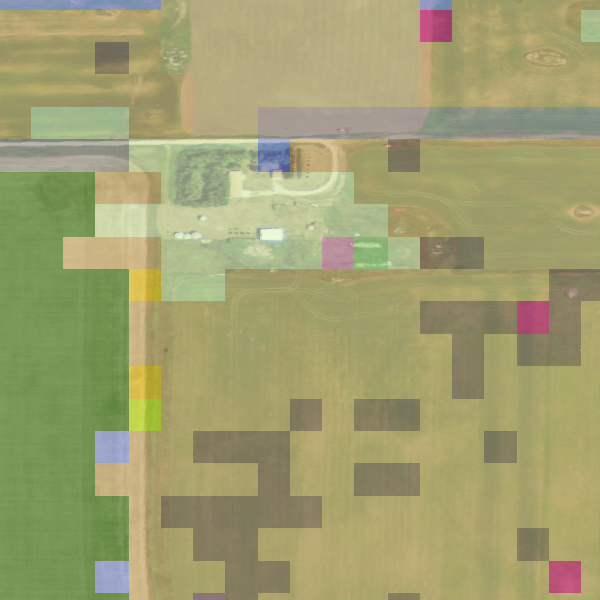
\includegraphics[width=\linewidth]{images/poor_labels_1.png}
      \caption{Mislabeled pixels.}
    \endminipage\hfill
    \minipage{0.32\textwidth}
      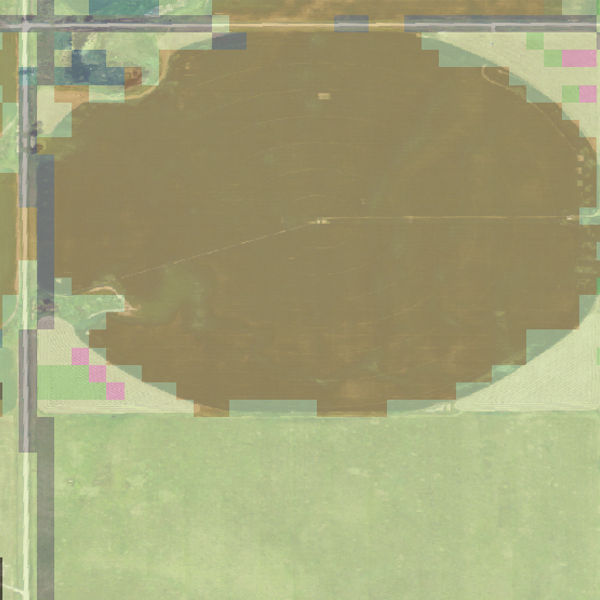
\includegraphics[width=\linewidth]{images/poor_labels_2.png}
      \caption{Clipped organic features.}
    \endminipage\hfill
    \minipage{0.32\textwidth}
      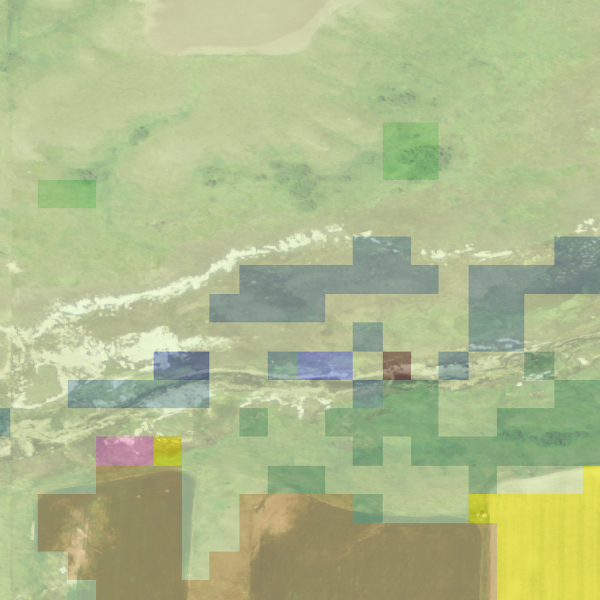
\includegraphics[width=\linewidth]{images/poor_labels_3.png}
      \caption{Fine features poorly represented.}   
    \endminipage 
  \end{figure}
\end{center}


Convolutional Neural Networks have been shown to be able to learn rough interpretations of geographical features given low resolution label data combined with high resolution orthoimagery imagery. 
\\

For this study, we will use the SegNet CNN architecture, along with imagery comprised of Red, Green, Blue, Near-Infrared (NIR) and Normalized Difference Vegetation Index (NDVI) image bands. We will also use image bands generated from the original 5 bands. The goal of this study is to discern whether the inclusion of several auxilary image layers aids in the classification accuracy and quantitative quality of these classifications.



\section{Related Work/Literature Review}

Much of previous orthoimagery segmentation and classification research has been focused on identifying roads and buildings, for use with mapping technologies such as Google Maps or Open Street Map. There seems to be very little research into the problem of generating classified segmentation for use with other applications such as natural resource surveying. Because per-pixel classifications of orthoimagery fall under the realm of scene recognition, we researched viable approaches to scene recognition. One of the notable works on scene recognition was SegNet. The SegNet publications outline a deep convolution encoder-decoder network which when applied to the CamVid data set produced good representations of features in the data set with relatively light computational requirements. The CamVid data set consists of ten minutes of high quality video imagery with corresponding semantically labeled images captured from a driving automobile. When applied to the CamVid data set, SegNet is able to produce high accuracy labels in real time. When searching for a staring point to begin with orthoimagery classification, it seemed worth while to see if the usefulness of SegNet was transferable to a new realm of sudy. The low computational requirements and the speed of the network were also attractive to minimise the upfront costs of hardware needed for training and testing a model.
\\

SegNet's architecture\cite{SegNet} consists of several corresponding encoder-decoder layers. Each encoder layer consists of a convolutional operation, followed by a batch normalization operation, followed by a Rectified Linear Units (RELU) operation, followed by a max-pooling operation. It is important to note that the max-pooling indices are saved for later use. Each decoder layer consists of an upsampling operation, a convolution operation, a batch normalization operation, and a RELU operation. A softmax classification layer is placed at the end of the network to compute the probabilities of classes. For the upsampling operation, the max-pooling indices from the encoder layer are used as the indices to unpool the inputs. This upsampling method is one of the unique qualities of SegNet. Upsampling in this manner allows for rapid training of a model because the decoder does not need to learn how to upsample the down-sampled filter windows of the previous layer. Effectively allowing us to produce per-pixel classifications at the same resolution as the input image.

\begin{figure}[!htb]
  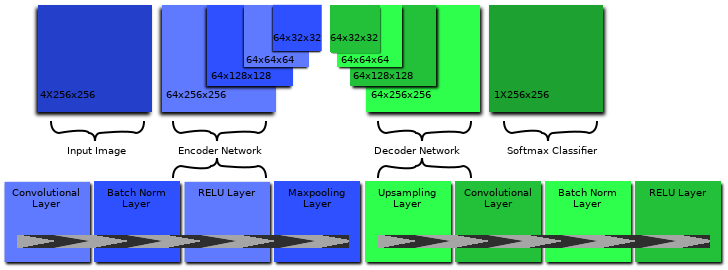
\includegraphics[width=\linewidth]{images/network.png}
  \caption{SegNet architecture. The encoder network consists of four sets of encoder layers of decreasing resolution. The decoder network consists of four sets of decoder layers of increasing resolution. The bottom row depicts the architecture of one encoder layer and one decoder layer. For every encoder layer, there is a matching decoder layer.}
\end{figure}
In more detail, each encoder layer performs a convolutionl operation to produce a set of feature maps. The feature maps are then batch normalized and a RELU operation is applied. Finally, a max-pooling operation is applied to the feature maps to ``reduce translational variance over small spacial shifts within the input image''\cite{SegNet}. The indices of the max-pooled samples are saved for use with a corresponding decoder layer. In each decoder layer, the corresponding indices are used to preform indice unraveling as a means of upsampling the feature maps. The upsampled feature maps are then convolved upon, batch normalized, and a RELU operation is applied. The resulting feature maps are then fed to a softmax classifier and per-pixel label-wise probabilities are computed. 


\section{Data Set Preprocessing}
As described above, our data sets consist of raw images from the National Imagery Program (NAIP), and land-use classification data from the National Agricultural Statistics Service (NASS). NAIP imagery is acquired at one-meter ground sample distance (GSD) and provides red, green, blue, and near infrared image layers \cite{NAIP}. Images from the NAIP data set are available for download via the EarthExplorer tool hosted by the United States Geographical Services. EarthExplorer allows users to query various geographical datasets and interfaces with a bulk data download application. Once the image data is downloaded, the GDAL library (Geospacial Data Abstraction Library) tooling is used to generate a set of shapefiles which are then uploaded to the NASS CropScape land use classification tool. CropScape allows users to upload points of interest as shapefiles and fetch land-use classification data for a region contained by the shapefile. Once the land-use classification data is downloaded, the GeoTiff files containing the data must be resized to match the resolution of the NAIP imagery files. GDAL, using the gdalwarp command, is used for this purpose. Because GeoTiff files are georectified, resizing the classification images does not offset pixels in the image and we do not need to worry about pixels in the resized image being anti-aliased or smoothed in some way which might produce invalid data. A script then slices the NAIP image and the NASS classifications into 256x256 pixel swatches, and stores each channel of the NAIP image in its own greyscale PNG file. The near-infrared layer is converted to a Normalized Difference Vegetation Index (NDVI) scaled from 0 to 255 (more on this is covered in the Architecture section). Classification images from NASS contain 255 different possible labels. In order to simplify these labels we grouped labels into one of two groups: Not-Water and Water which we use as our labels to predict. The breakdown of which NASS labels were grouped into each label can be seen in \textbf{Figure 5}. Each classification swatch is stored as a greyscale image. Images are stored in this manner to allow easy visualization of the images. Because the input image consists of four layers: red, green, blue, and NDVI - the NDVI layer is interpreted by image viewers as an opacity layer which would make manual inspection of swatches difficult. During training and testing, these sets of image swatches are loaded in batches and passed into the model.

\section{Auxilary Image Layers}
We will be examining two different types of auxilary image layers, a window-based gradient approach, and a window-based regression approach.

\subsection{Gradient Based Image Layer}
Using a sliding window, a gradient is computed by taking the scaled value between 0 and 255 of the the largest difference in pixel intensity within the window. The sliding window operates over one of the original image layers to produce an intensity value for each pixel in the image, excluding a small border that often forms when using window based techniques. The size of the border depends on the size of the sliding window. For all of our expiriments we will be using the NDVI layer as input to the gradient operation. We will also be using a window size of 8x8 pixels which results in an output image of 248x248 pixels. The other bands of our input images are clipped to the same size.

\subsection{Regression Based Image Layer}
Using a sliding window, we take the slope of the line calculated by taking the linear regression between two bands using the pixels that fall within the window. The sliding window operates over two of the original image layers to produce a value for each pixel in the image, excluding a small border that often forms when using window based techniques. The size of the border depends on the size of the sliding window. For all our expiriements we will be using the Red and Near-Infrared bands as input to the gradient operation. Our implementation is based on the paper Multi-scalar Analysis of Geospatial Agricultural Data for Sustainability which introduces a means of allowing larger sliding windows without the computational cost of scanning for them.\cite{Denton}. As, such our decision to use the Red and NIR bands is based on some of the insights from this study. We will also be using a window size of 8x8 pixels which results in an output image of 248x248 pixels. The other bands of our input images are clipped to the same size.

\begin{figure}
  \begin{tabular}[]{|p{2cm}|p{12cm}|}
  \hline
  Not-Water & Forest, Shrubland, Christmas Trees, Other Tree Crops, Deciduous Forest, Evergreen Forest, Mixed Forest, Woody Wetland, Fallow/Idle Cropland, Developed, Developed Open Space, Developed Low Density, Developed Medium Density, Developed High Density, Grass/Pasture, Corn, Cotton, Rice, Sorghum, Soybeans, Sunflower, Peanuts, Tobacco, Sweet Corn, Pop or Oat Corn, Mint, Barley, Durum Wheat, Spring Wheat, Winter Wheat, Other Small Grains, Double Crop Winter Wheat and Soybeans, Rye, Oats, Millet, Speltz, Canola, Flaxseed, Safflour, Rape Seed, Mustard, Alfalfa, Other/Non-hay Alfalfa, Camelina, Buckwheat, Sugarbeets, Dry Beans, Potatoes, Other Crops, Sugarcane, Sweet Potatoes, Misc. Vegitables \& Fruites \\ \hline
  Water & Water, Aquaculture, Open Water, Herbaceous Wetlands \\ \hline
  \end{tabular}
  \caption{Model classes to NAIP class breakdwon. Note that not all NAIP classes are represented in our data set as most of our images come from North Dakota and not all privided crops or land use types are common in state.}
\end{figure}


\begin{figure}
 \centering{
  \begin{tabular}[]{|p{2cm}|p{2cm}|p{2cm}|p{2cm}|p{2cm}|}
    \hline
    Not-Water & Water \\ \hline
     ~93\% & ~7\%  \\ \hline
  \end{tabular}
  \caption{Break down of class representation by percentage.}
 }
\end{figure}



\section{Architecture}

For the most part, our model encompasses a vanilla implementation of SegNet. The original SegNet model takes 4-band images as input. The first three bands correspond to the conventional red, green, and blue layers. The fourth band is a depth map scaled between 0 and 255. The fourth band in the image of our model is a Normalized Difference Vegetation Index (NDVI)\cite{NDVI} scaled between 0 and 255. The NDVI layer of our images is computed using the red and near-infrared layers of our source images using the following formula:  
\begin{figure}[!htb]
  \centering{
    $ NDVI = \frac{NIR-RED}{NIR+RED} $
  }
\end{figure}

NDVI is useful for tasks where vegitation is involved, this is due to the way near-infrared light reflects differently off of vegetation and non-vegetation. Optionally, a fifth auxilary image layer may be included - this will be either the Gradient based auxilary image, or the Regression based auxilary image.
\\

Another difference between our model and the original SegNet model, is varying convolutional kernel sizes. SegNet recommends a 7x7 convolutional kernel size. This seems to work well for the SegNet data set image size and its task, however such a large convolutional kernel reduces sensitivity to fine features and does not work as well in our much smaller images (smaller images means noticeably finer features than in the CamVid data set). We will be using a 3x3 kernel. The 3x3 kernel allows for detection of finer features than the 7x7 kernel. 

\section{Training and Evaluation}
Before training, a dataset of 2000 images is randomly partitioned into 90\% and 10\% splits. The model is then trained on 90\% of the available image swatches (1800 image swatches) in batches of 5 for 8 epochs. While training we save checkpoints every 100 steps. Post training we then select the checkpoint with the highest evaluation accuracy. The model is evaluated on 10\% of the available images (200 image swatches). Evaluating and training with k-fold cross validation is planned for the future but could not be implemented due to time constraints.

\section{Analysis}

\begin{figure}[!htb]
 \centering{
  \begin{tabular}[]{|l|l|}
    \hline
    Model Type & Accuracy \\ \hline
    Control (No Aux Image layer) & 92.3680\% \\ \hline
    Regression                   & 86.0488\% \\ \hline  
    Gradient                     & \textcolor{olive}{93.3380\%} \\ \hline     
  \end{tabular}
  \caption{Evaluation accuracy of model variants.}
 }
\end{figure}

\begin{figure}[!htb]
 \centering{
  \begin{tabular}[]{|l|l|l|} 
    \hline
    Model Type                   & No-Water Accuracy   & Water Accuracy \\ \hline
    Control (No Aux Image layer) & 96.8892\%  & 37.6272\% \\ \hline
    Regression                   & 89.7641\% & \textcolor{olive}{40.82367\%} \\ \hline  
    Gradient                     & \textcolor{olive}{98.5329\%} & 30.26023\% \\ \hline     
  \end{tabular}
  \caption{Evaluation per-class accuracy of model variants.}
 }
\end{figure}



As previously discussed, due to the nature of the dataset (poor quality of ground truth data) the overall accuracy statistic (\textbf{Figure 7}) alone is not sufficuient to judge performance. As such, we have also included the per-class accuracies (\textbf{Figure 8}) which allow for several more useful observations. Additionally, a quantitative comparison of the different model outputs proves useful for seeing differences in the quality of the classifications.

As seen in \textbf{Figure 7} the model that was fed the gradient auxilary image layer outperformed the other two models in terms of overall accuracy. We can see by examining \textbf{Figure 8} that this increase in accuracy appears to come from slighly increased per-class accuracy for No-Water, at the considerable cost of per-class Water accuracy. We can see this clearly in \textbf{Figure 9} where the Not-Water classification encroaches on areas which are clearly part of a water source (For an explanation on how to interpret the classification images see the Appendix: Interpreting Classification Images).

\begin{figure}[H]
  \centering{
    \fbox{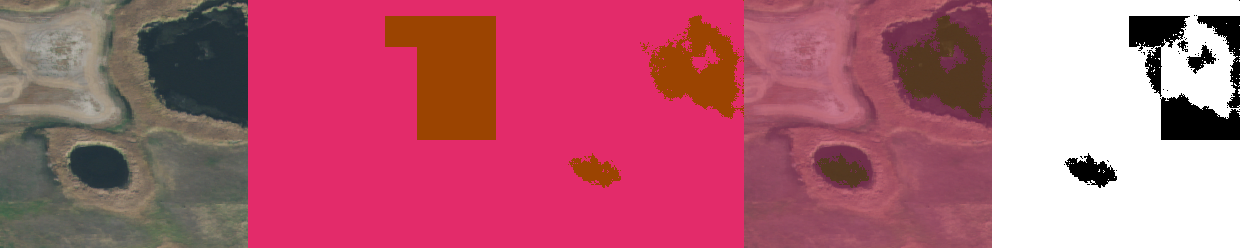
\includegraphics[width=\linewidth]{images/grad_104_loss_of_water_accuracy.png}}
    \caption{The generated classification eagerly selects Not-Water as the given class}
  }
\end{figure}

The model that was fed the regression auxilary image layer had a lower overall accuracy, but a higher per-class accuracy for Water. In \textbf{Figure 10}, \textbf{Figure 11}, and \textbf{Figure 12} we can see that the regression model output correctly classifies the small water source in the middle of the image. The cost for this are the number of missclassified artifacts throughout the generated image as compared to the output of the other two models.

\begin{figure}[H]
  \centering{
    \fbox{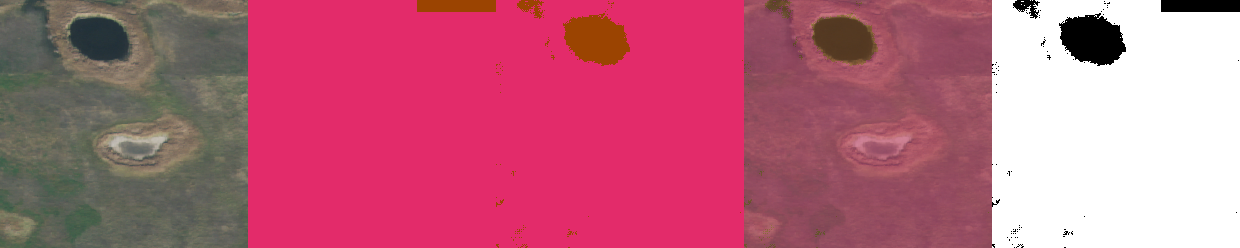
\includegraphics[width=\linewidth]{images/control_114_missing_secondary_water_source.png}}
    \caption{Control model output}
  }
\end{figure}
\begin{figure}[H]
  \centering{
    \fbox{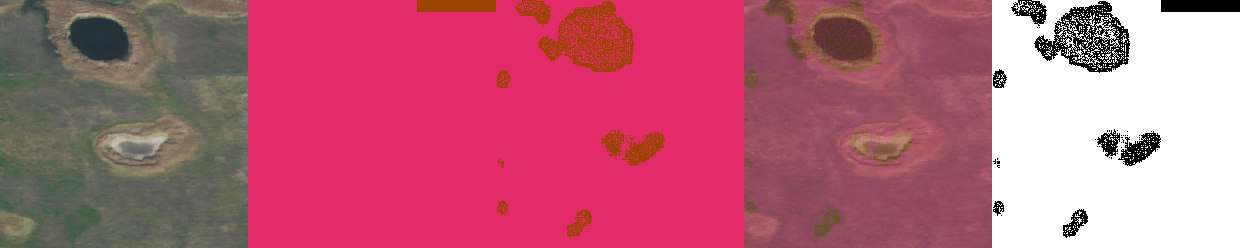
\includegraphics[width=\linewidth]{images/regression_114_missing_secondary_water_source.png}}
    \caption{Regression model output}
  }
\end{figure}
\begin{figure}[H]
  \centering{
    \fbox{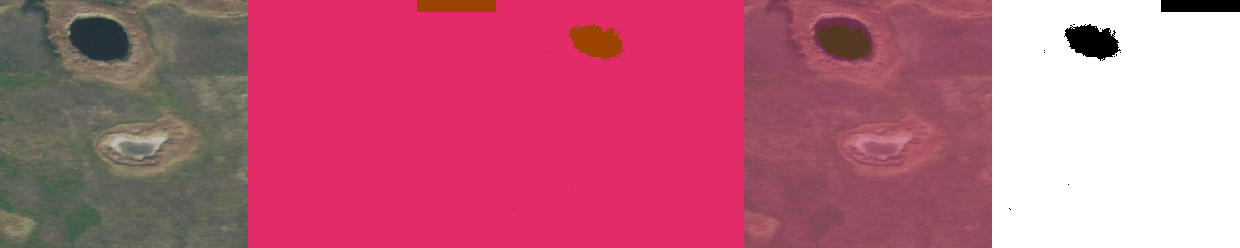
\includegraphics[width=\linewidth]{images/gradient_114_missing_secondary_water_source.png}}
    \caption{Gradient model output}
  }
\end{figure}

We have also seen many cases where the regression model's water classifications tend to include and respond more strongly to places where there is lots of vegitation along the coast of a water body as can be seen when comparing \textbf{Figure 13}, \textbf{Figure 14}, and \textbf{Figure 15}

\begin{figure}[H]
  \centering{
    \fbox{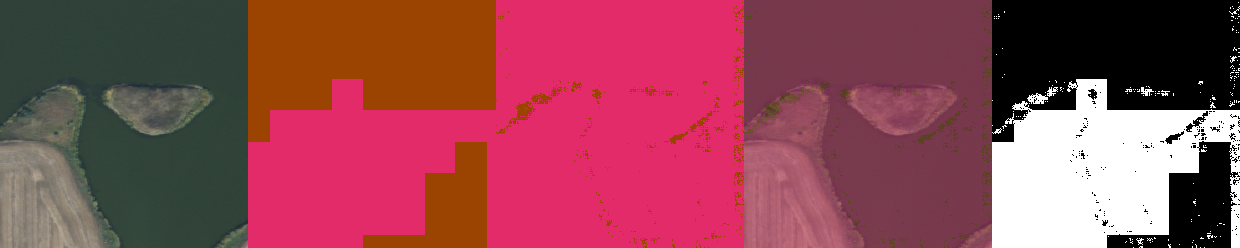
\includegraphics[width=\linewidth]{images/control_12_strong_waterline_response.png}}
    \caption{Control model output}
  }
\end{figure}
\begin{figure}[H]
  \centering{
    \fbox{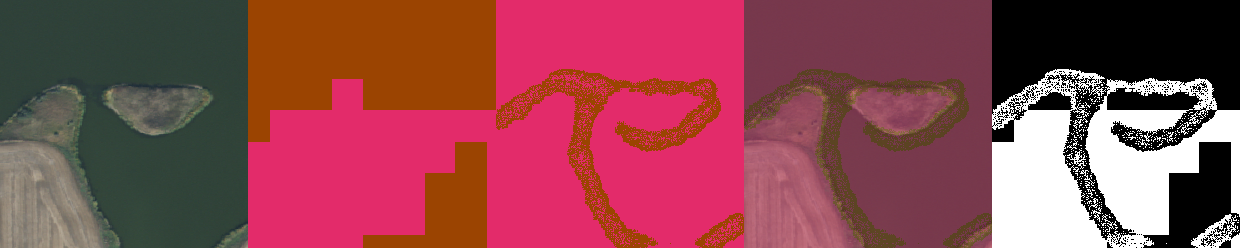
\includegraphics[width=\linewidth]{images/reg_12_strong_waterline_response.png}}
    \caption{Regression model output}
  }
\end{figure}
\begin{figure}[H]
  \centering{
    \fbox{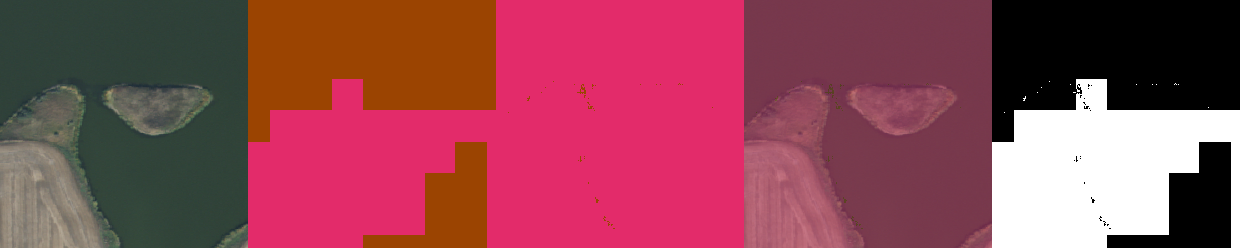
\includegraphics[width=\linewidth]{images/grad_12_strong_waterline_response.png}}
    \caption{Gradient model output}
  }
\end{figure}

Generally we have observed that the control model tends to under-estimate the size of small water sources. The gradient model tends to further underestimte the size of water sources when compared to the control model. Lastly, the regression model tends to vastly over-estimate the size of water bodies, particularly when there is a large source of vegitation surrounding the waterline. We attribute this over-estimation to the responses of the regression operation. When the regression operation is performed on the Red and NIR bands the response seems particularly high in areas with dense vegitation. Water itself is typically distinguished by its relatively now NIR reflectivity. As a result, the model may be using the border between the high responiveness of the regression image in places with vegetation and low responsivenes of the regression image in places with no vegetation - i.e. places with water.
\\

Finally, we would like to experiment more with the varying combinations of different window sizes used by the regression and gradient preprocessing steps. We hope that by finding optimal window sizes we may further the promsing results we have seen thus far. 

\section{Conclusion}

We have seen that the two types of auxilary image layers we have tested have aided the base model in varying ways. The gradient image layer aided the base model in correctly classifying more Non-Water pixels, often times overestimating the boundaries of the Non-Water features. The regression image layer has aided the base model in correctly classifying more Water pixels, similarly overestimating the boundaries of Water features - especially where there is moderate vegitation surrounding a Water feature.
\\

These conclusions lead us to believe that while the convolutional neural network may eventually learn decent representations of features on its own, the addition auxilary image layers, created by preprocessing the original image, can successfully guide the model to learn new features before reaching the point of overfitting the data.
\\

Further research may include determining if the positive results of this study are effected by window-based vs non-window-based techniques for generating auxilary image layers.


\newpage
\section{Appendix}

\subsection{Interpreting Classification Images}
\begin{figure}[!htb]
  \centering{
    \fbox{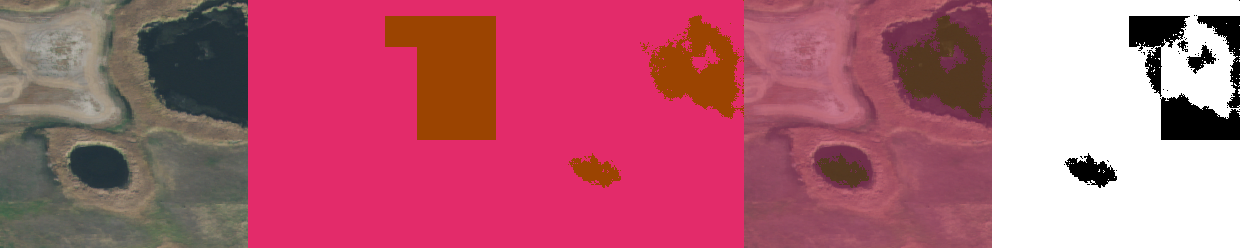
\includegraphics[width=\linewidth]{images/grad_104_loss_of_water_accuracy.png}}
    \caption{Legend - Pink: Not-Water, Brown: Water}
  }
\end{figure}

Our classification images are comrpised of five separate sections. The first two sections of the image are our input image and the ground truth image respectively. The third section shows the classification image output by the model. The fourth section is the input image overlaid with our generated classification image. The fifth section highlights differences between the ground truth and the generated classification image. White pixels indicate that the classifications matched. Black pixels indicate that the two images selected different classes at that pixel location. The fifth section is especially useful for illustrating the limitations of such low-resolution ground truths.  

 
\newpage
\bibliographystyle{plain}
\bibliography{mics_2018}

\end{document}

